\chapter{Tổng quan về bài toán và cơ sở lý thuyết}
\label{ch:ly-thuyet}

\section{Tổng quan về mô hình ngôn ngữ lớn}

Mô hình ngôn ngữ lớn là các mô hình học sâu được huấn luyện trên khối lượng văn bản lớn, có khả năng hoàn thành, tóm tắt, trả lời và sinh nội dung theo ngữ cảnh. Trong ứng dụng thực tế, LLM thường không đứng một mình mà được bọc bởi lớp ứng dụng: giao diện người dùng, kho tri thức, công cụ gọi ngoài, và chính sách an toàn. Khả năng ``làm theo chỉ dẫn bằng ngôn ngữ tự nhiên'' cũng chính là điểm yếu khi chỉ dẫn độc hại được đưa vào cùng kênh dữ liệu với chỉ dẫn hệ thống.

\section{Kiến trúc hệ thống ứng dụng mô hình ngôn ngữ lớn}

Một kiến trúc phổ biến là RAG: (1)~người dùng gửi câu hỏi; (2)~hệ thống truy hồi đoạn tài liệu liên quan; (3)~mô hình sinh câu trả lời dựa trên ngữ cảnh truy hồi và chỉ dẫn hệ thống. Các thành phần bổ sung có thể gồm bộ lọc đầu vào/đầu ra, nhật ký kiểm toán, và lớp ủy quyền nguồn tài liệu. Trong đề tài, kiến trúc lab dùng Mock LLM Provider (hành vi tất định, không gọi mạng) và truy hồi lexical (SQLite FTS5/BM25) thay cho vector store, nhằm ưu tiên tính tái lập và kiểm thử.

\section{Các rủi ro an toàn trong hệ thống LLM}

\subsection{Prompt injection}

Prompt injection là kỹ thuật khiến mô hình ưu tiên chỉ dẫn của kẻ tấn công hơn chỉ dẫn hệ thống, ví dụ yêu cầu ``bỏ qua mọi chính sách trước đó''. Dạng gián tiếp xảy ra khi chỉ dẫn độc hại nằm trong tài liệu/email được nạp vào ngữ cảnh RAG~\cite{owasp_llm_top10}.

\subsection{Rò rỉ dữ liệu và thông tin nhạy cảm}

Hệ thống có thể phát tán PII, bí mật giả định, hoặc nội dung nội bộ nếu đầu ra không được kiểm soát, hoặc nếu gói bàn giao chứa file log/dữ liệu thô (JSONL, \texttt{result.json}, cơ sở dữ liệu tạm).

\subsection{Đầu ra không an toàn}

Ngoài rò rỉ, đầu ra có thể chứa hướng dẫn lạm dụng, nội dung độc hại, hoặc khẳng định sai sự thật. Lớp output guard và chính sách từ chối an toàn nhằm giảm rủi ro này ở mức rule-based lab.

\subsection{Sai lệch hoặc nội dung không đáng tin cậy}

Mô hình có thể ``ảo giác'' hoặc bị thao túng bởi ngữ cảnh độc. Cơ chế provenance/trust và giới hạn nguồn tài liệu phía máy chủ giảm phụ thuộc mù quáng vào nội dung truy hồi.

\subsection{Rủi ro từ dữ liệu, công cụ và thành phần tích hợp}

Archive lồng nhau, đường dẫn Windows/Unix không an toàn, ZIP không chuẩn, và phụ thuộc phần mềm chưa quét lỗ hổng đều tạo rủi ro vận hành. Đề tài coi kiểm tra gói phát hành là một lớp kiểm soát ngang hàng với guard runtime.

\section{Nguyên tắc kiểm soát an toàn}

\subsection{Kiểm soát đầu vào}
Lọc và phân loại prompt theo mẫu/rule; chặn hoặc gắn cờ injection, jailbreak, yêu cầu trích xuất nhạy cảm.

\subsection{Kiểm soát đầu ra}
Rà soát chuỗi nhạy cảm, chỉ dẫn rò rỉ; sanitize hoặc block theo chính sách.

\subsection{Quản lý chính sách và quyền truy cập}
Allowlist/denylist đóng thế giới; nguồn tài liệu được máy chủ quyết định; không để ứng dụng tin tưởng mù quáng đường dẫn do client chỉ định.

\subsection{Ghi nhận sự kiện và truy vết}
Log quyết định guard với mã lý do ổn định; tránh ghi nội dung bí mật thô ra kênh công khai.

\subsection{Kiểm thử và xác minh}
Bộ case red-team tổng hợp, kiểm thử tự động, và (ở lớp phát hành) verify trước khi publish.

\section{Một số tiêu chuẩn và tài liệu liên quan}

Nhóm tham chiếu OWASP Top 10 for LLM Applications~\cite{owasp_llm_top10} và OWASP LLMSVS~\cite{owasp_llmsvs} như khung phân loại rủi ro và kiểm soát. Các công trình về tấn công/phòng thủ RAG (ví dụ PoisonedRAG~\cite{zou2024poisonedrag}) được ghi nhận ở mức xác minh tồn tại nguồn; báo cáo không trích số liệu chi tiết từ các bài chưa đọc toàn văn (xem phụ lục).

\begin{figure}[H]
\centering
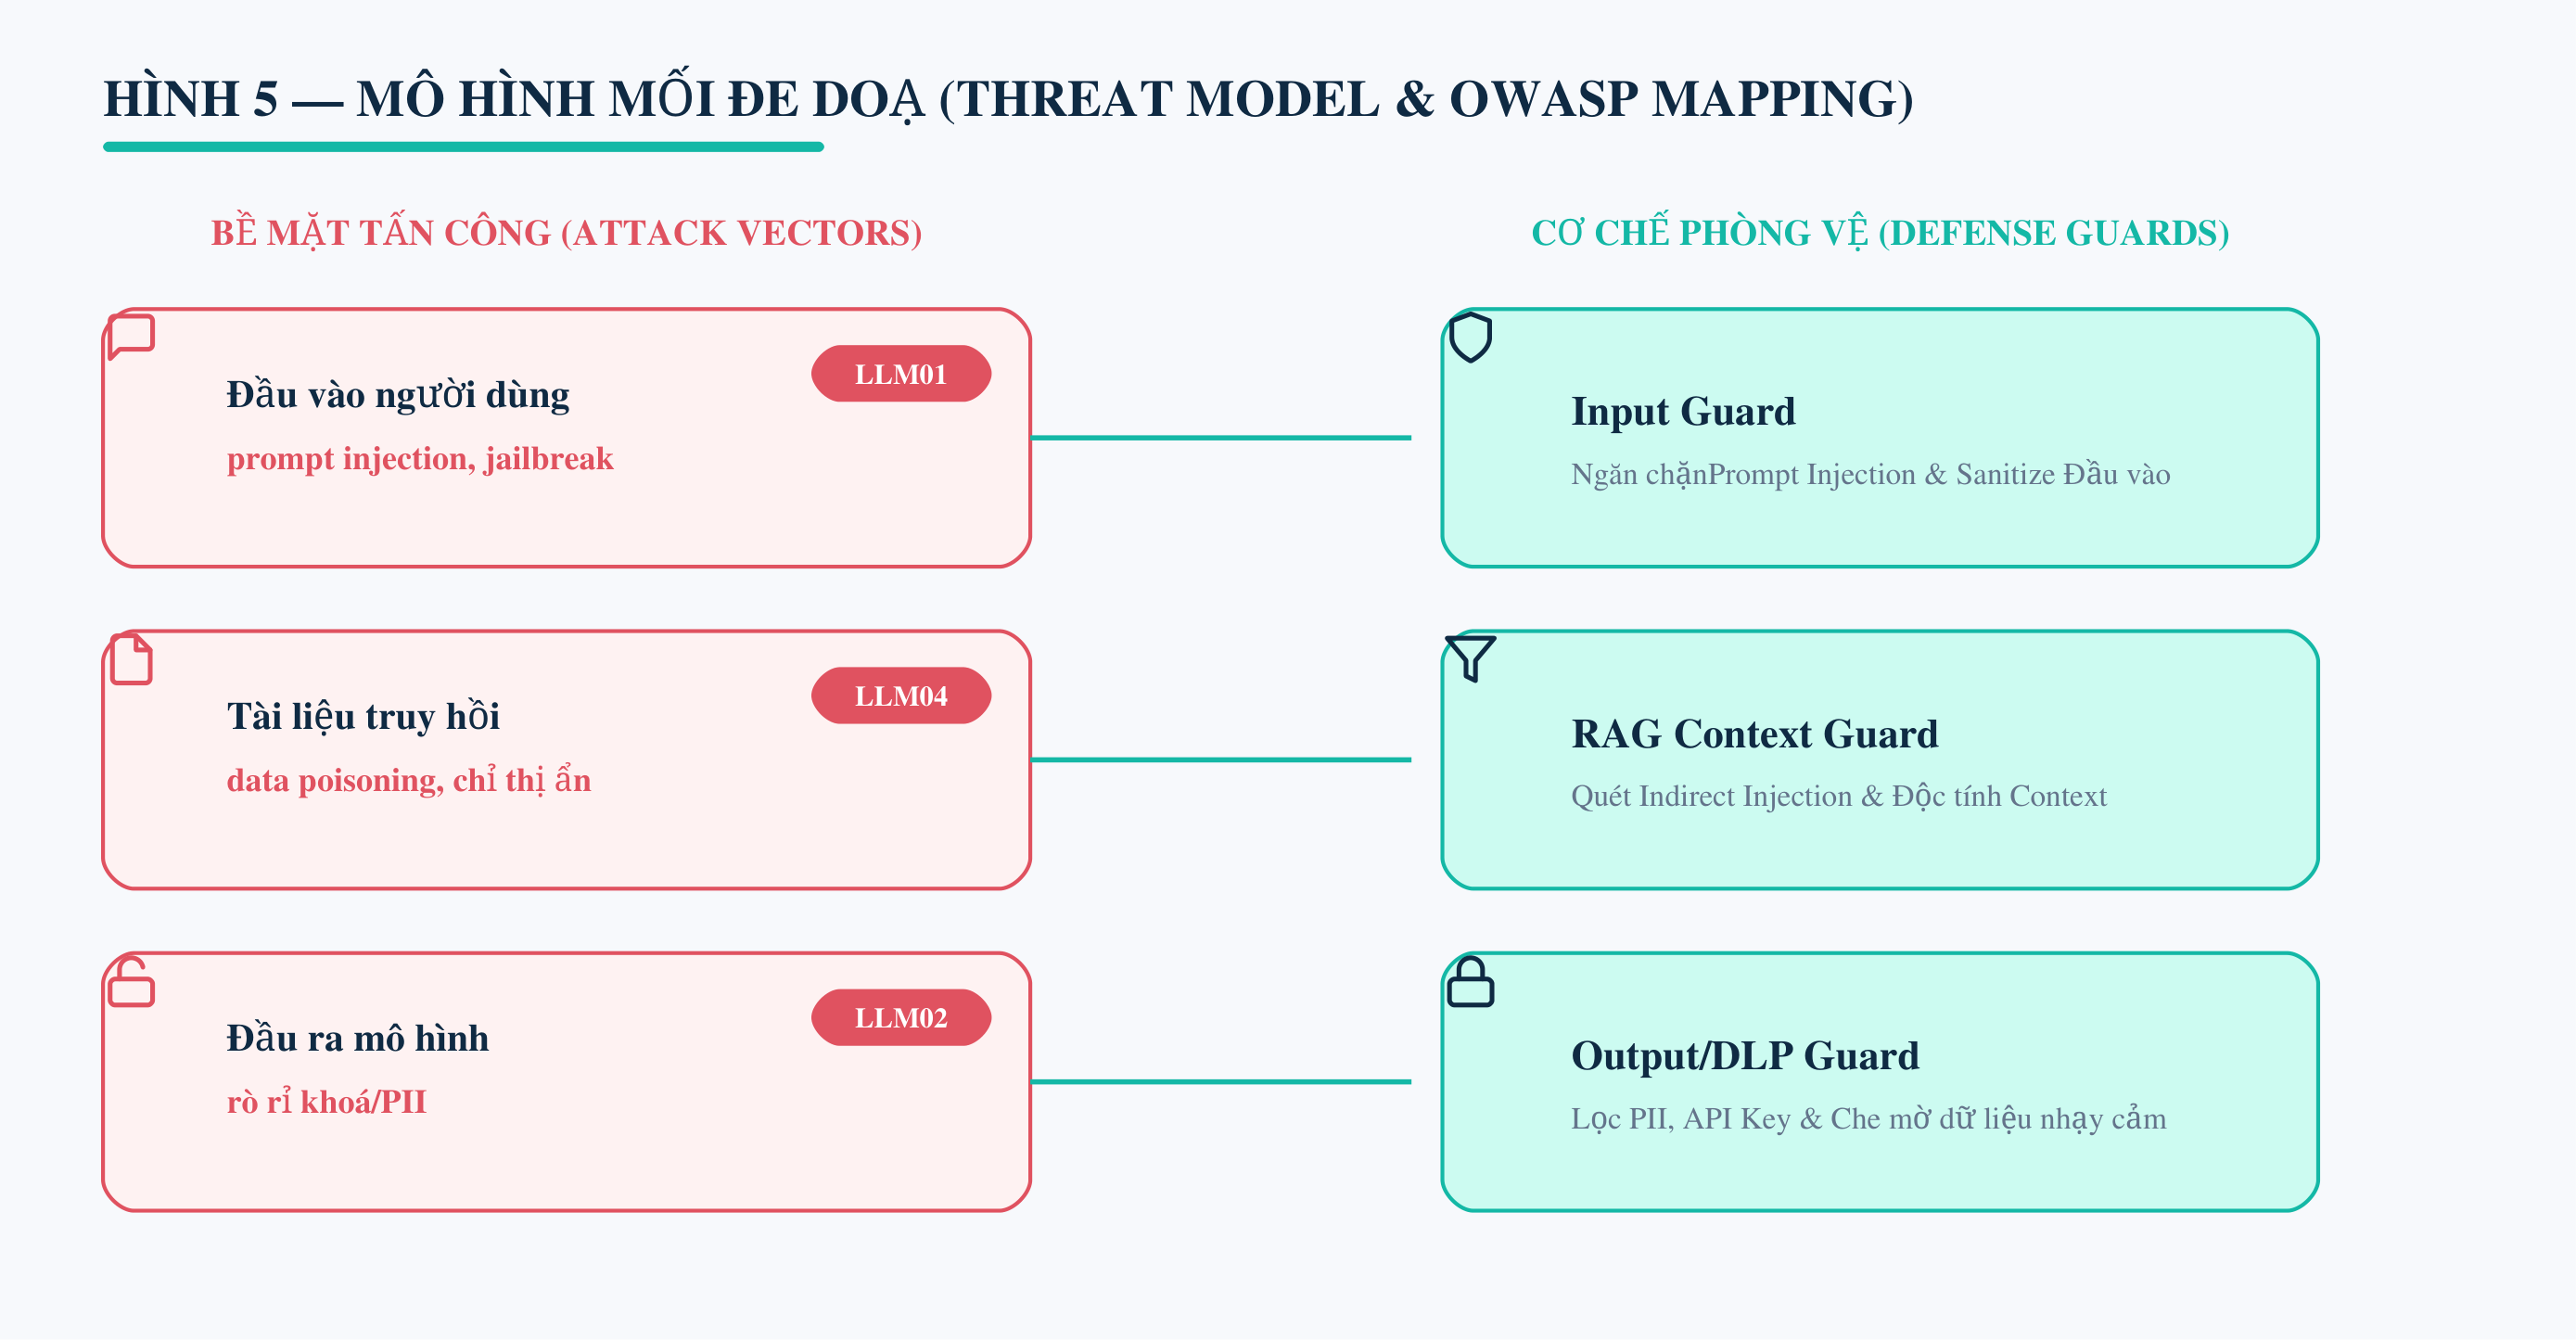
\includegraphics[width=\linewidth]{figures/fig-threat-model.png}
\caption{Mô hình mối đe doạ: ba bề mặt tấn công và guard phòng vệ tương ứng}
\label{fig:threat-model}
\end{figure}

Hình~\ref{fig:threat-model} ánh xạ ba bề mặt tấn công của hệ thống RAG/LLM sang
lớp guard xử lý và mục tương ứng trong OWASP LLM Top 10: đầu vào người dùng
(prompt injection, jailbreak --- LLM01) do Input Guard xử lý; tài liệu truy hồi
(data poisoning, chỉ thị ẩn --- LLM04) do RAG Context Guard xử lý; và đầu ra mô
hình (rò rỉ khoá, PII --- LLM02) do Output/DLP Guard xử lý.

\section{Kết luận chương}

Chương này xác lập nền tảng: LLM/RAG mang lại năng lực mới nhưng mở rộng bề mặt tấn công; kiểm soát cần đa lớp (đầu vào, ngữ cảnh, đầu ra, gói phát hành) và phải đo được bằng kiểm thử có kiểm soát. Chương tiếp theo chuyển sang phân tích yêu cầu và thiết kế hệ thống của đề tài.
